\chapter{Technical Approach} \label{chapter:technicalApproach}

\section{Introduction}
\paragraph{}
Running an accurate detection in real time on a smartphone is a difficult task as the literature review of Chapter \ref{litreview} already showed. Due to the limited time and scope of this work, we will not try to revolutionize this field, and focus on building on existing methods and taking advantage of the specificity of our task: traffic signs detection.

In this chapter we will first list the assumptions we took and expose their importance. We will then go deeper in the implementation by describing our output layer by showing its difference from other widely used networks and what are the benefit we are targeting with these changes. Once the output head is defined we will present our backbone structure and finish by detailing some implementation details such as the data management.

\section{Assumptions} \label{Assumptions}
\paragraph{}
Well known architectures for object detection, such as MobileNet-SSD \cite{sandler2018mobilenetv2}, already achieve great performance on mobile. It is out of scope of this work to improve over it for general object detection, but our task of object detection has some specificity that we can leverage to make things easier for detection. In this section we will present you those different assumptions and their motivations.

\subsection{Aspect ratio} \label{assumptionAspectRatio}
\paragraph{}
The first assumption we are going to take is that given a sign class, the aspect ratio of the object we are going to detect is always the same. Traffic signs follow well-defined standards, and if their size may change from one road condition to the other, their shape will stay the same. Due to perspective transformation they may appear with slightly different aspect ratio, but the sign giving information to the drivers, they are always facing it and so suffer from very small deformation when being seen from the windshield.

Neural network have already been proven to be very good at predicting the aspect ratio of the shape they are trying to detect. However, when using smaller backbone network, this prediction tend to become less accurate. This is often the case on models like tiny-yolo \cite{yolov3}. This makes us realize that the network spends a fair amount of effort computing those values accurately. Removing those completely will reduce significantly the complexity of the task while having only minor impact on the accuracy in our task.

\subsection{Position accuracy}
\paragraph{}
Following the same idea as during Section \ref{assumptionAspectRatio}, the accurate position is also something difficult to predict. Most of the detection networks, such as SSD \cite{liu2016ssd}, predict a given number of bounding boxes for an area, each having their own classes and position offset. Setting this position offset to the center of the detection area will make the task easier and reduce the load on the backbone network.

However, to maintain accuracy this requires to have smaller detection zone, showing an important trade-off here. Although this note is mostly important for deep backbone models that have a lot of convolution layers before the final output, having a small backbone network will mitigate this effect.

\subsection{Size accuracy}
\paragraph{}
Common one shot detection models like SDD \cite{liu2016ssd} and Yolo \cite{yolov3} use different layers to predict objects of different size. Each layers then predict variation around a given anchors size. Computation of Intersection over Union (IoU) with these default anchors showed that on our data, a small set of anchors achieved very high score. This allowed us to further reduce the complexity by removing the size prediction and directly use the anchor size as a prediction shape.

\subsection{Task complexity}
\paragraph{}
In addition to all the simplification given previously, we assume that our task is an easy case. Traffic sign are made to be easy to seen by human, they usually use bright colors and clear shapes. In addition, results from \cite{de1997road, janssen1993hybrid, besserer1993shape} show that simple pixel operation like color threshold and edges detection give good results on sign detection task. Showing us that a few layer backbone should perform great on this task.


\section{Detection layer}
\subsection{Intuition}
\paragraph{}
Following the assumptions given during Section \ref{Assumptions}, we are looking for a detection layer that is less generic than widely used ones, such as SSD \cite{liu2016ssd}. This loss should allow us to make the underlining function simpler and so easier to approximate with a neural network, which will allow us to use smaller network to approximate it.

Convolution operation are very good at doing pattern matching. Weights visualization techniques, such as the one presented in \cite{yosinski2015understanding} show that networks are very good at understanding the shape of an object. However, predicting the object size, even if possible as already done by different models \cite{yolov3, liu2016ssd, ren2015faster}, is a more complex process for this kind of operation.

Removing the need of this prediction is, however, not harmful to our traffic sign detection task, as explained in Section \ref{Assumptions}. Simplifying the task to classification of given bounding box regions of the images will strongly decrease the load on the backbone network complexity resulting in performance gain.

\subsection{Detection computation}
\paragraph{}
We chose to make our detection approach very similar to the one presented in SSD \cite{liu2016ssd}. We will predict classification and position of signs at different levels of our network and for each head each cell will predict one class.

Similarly, to the approach presented in \cite{liu2016ssd}, each output cell predict one bounding box with its class. This set of classes to predict also include the background in addition to the classes you want to detect to allow a common multi class classification setting with the use of a soft-max activation function on each cell.

However, our approach differs to the one they propose in that we do not choose between different anchors for each cell, and we do not predict the variation of shape and position around these anchors.

This modification leave us with a very light version of SSD, reduced to its core idea.

\subsection{Loss function}
\paragraph{}
The training objective we chose for this architecture is derived from the SSD training loss \cite{liu2016ssd}. We use here a very similar classification loss, based on soft-max loss for each cell.

\begin{align}
     Loss(x,c) = \sum_{i \in Pos} x_i - \sum_{i \in Neg} x_i
\end{align}{}
\[
    \text{with } Pos = \left\{ i | c_{i0} = 0 \right\} \text{ and } Neg = \left\{ i | c_{i0} = 1\right\}
\]

However, the imbalance between positive samples, $Pos$, and negative ones, $Neg$, is large so instead of relying on every sample we only select the most important negative one using the well know methods of hard negative mining. Instead of computing the loss on all the negative samples, we reduce it to the worst one, the one with the higher confidence. We choose here a $3:1$ negative to positive maximum ratio. This value have shown to prevent most of the negative predictions while not confusing the network on the detection task.

\subsection{Anchors}
\paragraph{}
To make detection easier, we pushed the concept of anchors forwards. The anchors are no longer base shape that the network can change. They are actual boxes that the network is forced to use for its prediction. This lead to a large loss of the general object detection task, but as we already discussed in this Chapter, this loss is acceptable in our case.

We selected a set of five different anchors, giving Intersection over Union (IoU) of $75.28\%$ in our ground truth data. Each anchor is predicted by a different head, the smaller anchors being predicted first in the network and the largest at the end, so they can take advantage of a larger activation area. The anchors we used during this study are given on Table \ref{tab:anchors}. More information about the anchors and how they are affected by the general architecture of the model is given on Chapter \ref{chapter:resutls}, Section \ref{sec:detectionLayerPos}.

\begin{table}[]
    \centering
    \caption{Anchors box chosen for detection}
    \begin{tabular}{|l|c|c|c|c|c|}
        \hline
        Anchors size & $3\times3$ & $5\times5$ & $7\times7$ & $12\times12$ & $21\times21$ \\
        \hline
    \end{tabular}
    \label{tab:anchors}
\end{table}{}

\section{Backbone}
\paragraph{}
This aspect of the the network will be more broadly covered in Chapter \ref{chapter:resutls}, where we are going to explain and justify all the different choices we made for this architecture. However, we are going to describe here the different building blocks we tried.
\subsection{Compute Block}
The main structure of the network is composed of stacked computation block. We explored different type of block during this study, and evaluated their computational efficiency by comparing their speed and accuracy. All the block share common property. They all use a ReLu6 \cite{sandler2018mobilenetv2} activation function, batch normalization \cite{ioffe2015batch} and dropout \cite{srivastava2014dropout}. The difference is on the way they do the internal computation.
\subsubsection{Convolution block}
The first type of block is the very basic 2D convolution, illustrated by Figure \ref{fig:convblock}. It is simple but have shown great results in the past and even if it has received multiple improvements, it is still a very good base line.
\subsubsection{Residual block}
The second block is a residual block \cite{szegedy2017inception}. Residual block allows to reduce much of the gradient vanishing problem, and so allows building a deeper network. This is not our goal here as we want to maintain a small size, but this could improve training efficiency at a minimal cost. This block is illustrated in Figure \ref{fig:resblock}.
\subsubsection{Inverted residual Bottleneck}
The Inverted residual Bottleneck block was introduced by MobileNetv2 \cite{sandler2018mobilenetv2} as structure tailored to run on mobile devices. It is composed of a first expansion layer, a 2D convolution with kernel $(1,1)$, followed by a depth wise 2D convolution with kernel $(3,3)$, and the final outcome is given by projection layer, a 2D convolution with $(1,1)$ kernel. All of that are bundled in a residual block. A graphical representation of this block, From MobileNet v2 paper \cite{sandler2018mobilenetv2}, is provided on Figure \ref{fig:invertedbottleneckblock}.

\begin{figure}
  \begin{center}
    \begin{subfigure}[t]{.24\linewidth}
      \centering
      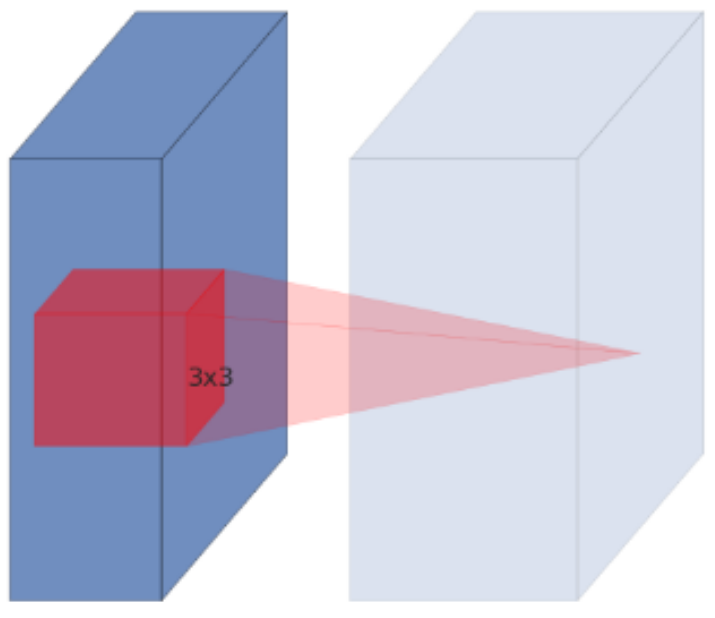
\includegraphics[width=.8\linewidth]{figures/mobilenetv2_conv.png}
      \caption{2D Convolution block}
      \label{fig:convblock}
    \end{subfigure}
    \begin{subfigure}[t]{.24\linewidth}
      \centering
      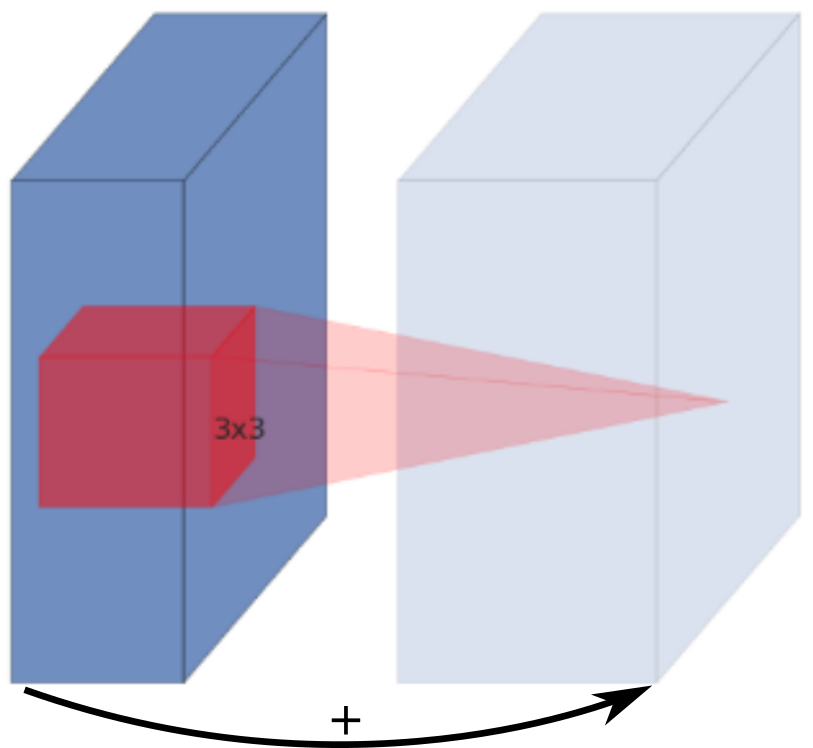
\includegraphics[width=.8\linewidth]{figures/mobilenetv2_resnet.png}
      \caption{Residual convolution block}
      \label{fig:resblock}
    \end{subfigure}
    \begin{subfigure}[t]{.5\linewidth}
      \centering
      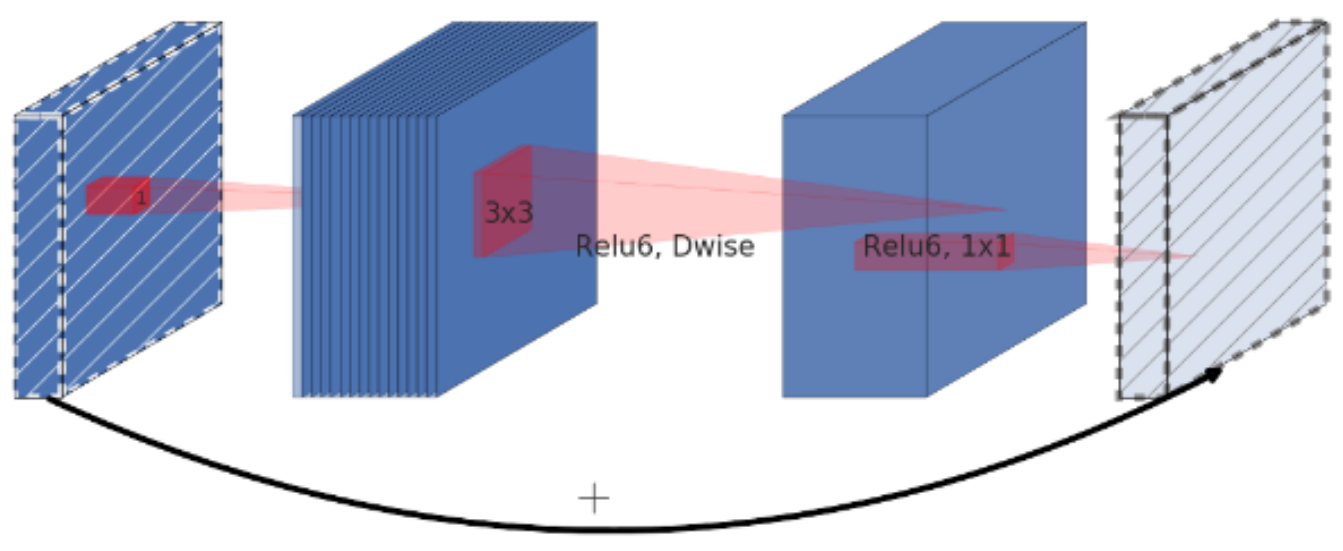
\includegraphics[width=.99\linewidth]{figures/mobilenetv2_inverted_residual_botleneck.png}
      \caption{Inverted residual block \cite{sandler2018mobilenetv2}}
      \label{fig:invertedbottleneckblock}
    \end{subfigure}
    \caption{Graphical representation of the different block used in this study, Illustrations from MobileNet V2 paper \cite{sandler2018mobilenetv2}}
  \end{center}
\end{figure}


\section{Training}
\subsection{Classes}
\paragraph{}
Our architecture is capable of being trained for multiple sign class, but in the context of this project we are mainly interested in one class, US diamond warning signs. Some example of such signs are available on Figure \ref{signExample}.

\begin{figure}
  \begin{center}
    \begin{subfigure}[t]{.3\linewidth}
      \centering
      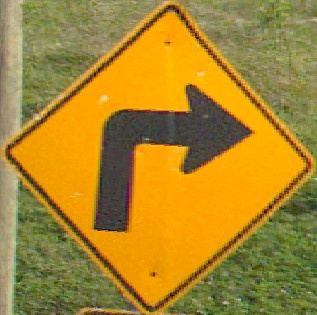
\includegraphics[height=0.8\linewidth]{figures/W1-1_R.jpg}
      \caption{W1-1}
    \end{subfigure}
    \begin{subfigure}[t]{.3\linewidth}
      \centering
      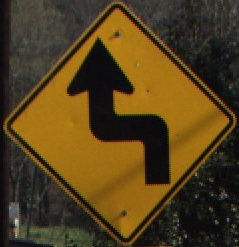
\includegraphics[height=0.8\linewidth]{figures/W1-3_L.jpg}
      \caption{W1-3}
    \end{subfigure}
    \begin{subfigure}[t]{.3\linewidth}
      \centering
      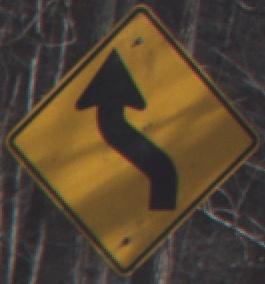
\includegraphics[height=0.8\linewidth]{figures/W1-4_L.jpg}
      \caption{W1-4}
    \end{subfigure}
    \caption{Example of US diamond warning signs, with there MUTCD sign class.}
    \label{signExample}
  \end{center}
\end{figure}

We chose not to aggressively ask the network to classify each sign directly into there MUTCD code as this task is much more difficult than only detection and can be handled with more accuracy by a specialized network. In addition, this strategy allow to reduce the input size. This smaller input size may make it impossible even for human to tell which MUTCD class the sign is, but is enough to say that there is a sign there, which is what we care about in this work. Once the sign is detected the image can be cropped at full resolution and given to a classification algorithm.

This approach may look very similar to the region proposal network of RCNN \cite{girshick2014rich}, and it is when you use only one class. However, when other classes are added this similarity get less clear. For example, you may want to add a stop sign class that does not require any other processing, or a speed limit class that will require specific digit detection algorithm.

\subsection{Data} \label{data_pres}
\paragraph{}
During this research, a large variety of data have been used. All this data were manually annotated by our research team and may be the subject of a later publication. The image were collected using either smartphone mounted on the windshield or externally mounted high resolution camera. Most of the images were collected in the north of the state of Georgia or around Nashville, over a large period of time.

This data set contains a large variety of  luminosity conditions and different seasonal background changes. However, it is important to note that this data set does not cover all the possible cases. First in the data collection regions, most of the rural areas are populated by trees, which represents most of the background of our images. In addition, the image collection was not the main purpose of the trip to those rural areas. As a result certain weather conditions such as rain are not widely present in the data. Data augmentation and generalization capabilities of the network may allow us to overcome such limitations, but without good testing data it would be difficult to assess those.

More information about the data are given in Appendix \ref{data}.

\subsection{Data generation} \label{sec:dataGen}
\paragraph{}
The data presented in Section \ref{data_pres} is a great source of information and are very important to this study, but they do not have enough samples to train a new model end to end correctly. To solve that issue we decided to rely on generating artificial data.

Our goal on this task was not to get photo realistic data, as they are not very realistic at very low resolution as we plan to use here, and are not needed. We want the network to use this data to get a broad understanding of what it should look for, on a very generic basis. To meet this goal we chose to train our model to detect yellow squares rotated by $45\deg$. The data we generate to meet this goal are far from any realistic image or even the real traffic sign we want to detect. An example of the generated image is given on Figure \ref{fig:fake_im_ex}. These images are generated following a very simple procedure, first the background is set to average pixel value of the real dataset from Section \ref{data_pres}. Then $500$ random polygons are drawn on top of it, starting with big ones and getting smaller and smaller. These polygons are convex and have between three and ten vertices. They are sampled by randomly choosing the angle and distance of each vertex regarding the center, while the color is randomly sampled from the color distribution observed in the real dataset. The goal of this generation is to create lot of different edges of similar color as in real live and to provide a not flat background to the target shapes. Over this background are then added the rotated yellow squares. Five such shape are added on each image, their sizes are sampled from the anchors size of the model, and colors are sampled following a normal distribution centered on yellow. The centers of the shapes are selected not to have large overlap with the edges of the image and to prevent any overlapping on each other. To prevent the model to learn to detect yellow objects we then add three not rotated square that otherwise follow the same logic as previously.

\begin{figure}
    \centering
    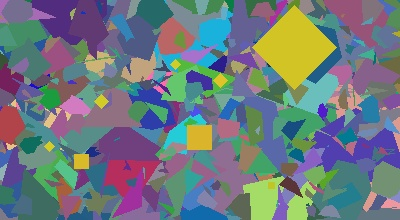
\includegraphics[width=0.5\linewidth]{figures/fake_data_ex.jpg}
    \caption{Example of artificially generated data}
    \label{fig:fake_im_ex}
\end{figure}{}

Using this logic we generated $20,000$ images and annotations to be used for our experiments.

\paragraph{}
We also considered replacing this pretraining data by a first training on a classification task. But we finally considered this step as not bringing enough benefit. First because training on sign classification will not bring much help as it will just teach the network to focus on the pictograph in the sign, not the sign itself. In addition, we could have used more generic dataset such as CIFAR 10 \cite{krizhevsky2009cifar10}, but we considered our model to be too shallow to learn useful features from such a training. The fact that the prediction is computed at different layers was also a problem to that idea. In conclusion, we decided that a first training on a classification task would not bring as much improvement as artificially generated data could.


\subsection{Data augmentation and prepossessing}
\paragraph{}
As it is common in deep learning, overfitting often arise on large networks. There is many different ways to prevent that. Some directly in the network, such as dropout \cite{srivastava2014dropout} that disable some connections in the network during training, or batch normalization \cite{ioffe2015batch} that normalize the output of each layer, improving training speed and mitigating the effects of overfitting. 

We applied these two methods to our network, but it is not enough to skip data augmentation entirely. Data augmentation was done using the classical approach, linear transformation of the image. This random transformation changes the image by applying random zoom in/out, shift and vertical symmetries. Rotation and shear were excluded from the data augmentation as they may result in change of the bounding box shape that depends on the actual object shape is are hard to predict. We also applied a color transformation to the image, by changing the brightness in order to simulate different lighting conditions.

\subsection{Architecture search}
\paragraph{}
In Chapter \ref{architectureSearch}, we presented different strategies to perform architecture search. Because of the lack of public implementation of this type of optimization strategy, and because of the size of our model, we chose to go for a broader way to explore meta-parameters. We used the classical grid search approach to this problem. As our model is able to be trainned in about an hour, such an approach does not cause any problem.

We used this the same way as NetAdapt \cite{yang2018netadapt} to fine tune the global architecture defined previously. This approach allowed us to get the relevant number of filters of each layer as well as tuning the dropout strategy to use.

In addition, similarly to ENAS \cite{pham2018efficient}, we implemented a parameters sharing process, allowing to save a lot of time on some grid search tasks.

